\section{Internal Diagnostics and Reproducible Workflow}
\label{app:internal}

Internal diagnostics evaluate whether the fitted model is consistent with its likelihood,
parameterisation, and data inputs. This appendix provides a reproducible structure for
detailed case-study reporting. Generic computation should live in R packages; case-study
scripts should load inputs, call package functions, record software versions, and write
tables and figures into the content files below.

\subsection{Required R Packages}

\begin{table}

\caption{\label{tab:internal-libraries}Required R packages for internal diagnostics.}
\centering
\begin{tabular}[t]{llll}
\toprule
package & role & tier & installed\\
\midrule
knitr & Knit template; format LaTeX tables & core & 1.51\\
r4ss & Read SS3 output; summarise convergence and likelihood components & run\_code & 1.53.0\\
sstruth & curveSS, diagSS, ssU, ssLen, ssRunSummary, residual plots & run\_code & 0.0.0.9020\\
diags & CPUE diagnostic summaries via sstruth::ssU & run\_code & 2.2.1\\
ggplot2 & Likelihood, residual, and recruitment-deviation figures & run\_code & 4.0.3\\
\addlinespace
reshape2 & Data reshaping for diagnostic plots & run\_code & 1.4.5\\
ss3diags & SSrunstest and ssruns\_sig3; CPUE runs-test plots with 3-sigma limits & run\_code & 1.10.2\\
FLRebuild & Fallback curveSS if sstruth unavailable & planned & 0.1.0\\
ss3om & Fallback readFLSss3 via readTruth (optional) & planned & 0.5.3.9004\\
\bottomrule
\end{tabular}
\end{table}



\subsection{Inputs}

Record the accepted model run, principal sensitivities, software versions, and data
objects used to create this appendix.

\begin{table}

\caption{\label{tab:internal-inputs}Internal diagnostics inputs.}
\centering
\begin{tabular}[t]{ll}
\toprule
item & value\\
\midrule
Assessment ID & sma-ss3-2026\\
Model class & SS3\\
SS base directory & P:/rfmo/iccat/2026/shark/Analysis/ss3\\
Scenarios & Scenario\_1/Sc1\_Base, Scenario\_2/Scn02\_base, Scenario\_3/Sc3\_Base\\
Reference scenario & Scenario\_1/Sc1\_Base\\
\addlinespace
SS version & 3.30\\
R version & 4.4.2\\
r4ss & 1.53.0\\
ss3diags & 1.10.2\\
sstruth & 0.0.0.9020\\
\addlinespace
diags & 2.2.1\\
FLRebuild & 0.1.0\\
ss3om & 0.5.3.9004\\
Run code & TRUE\\
\bottomrule
\end{tabular}
\end{table}



\subsection{Standard Checks}

The minimum internal checklist should include:

\begin{itemize}
  \item convergence status, maximum gradient, Hessian status, and parameters near bounds;
  \item likelihood components and evidence for conflicts among data sources;
  \item residual diagnostics for indices and composition data;
  \item effective sample size diagnostics for composition data;
  \item likelihood profiles or equivalent information-content diagnostics for advice-relevant quantities;
  \item recruitment deviations and whether stock--recruitment assumptions are informed by data;
  \item process-error diagnostics: residuals versus time, biomass, ACF, and distributional properties (Appendix~\ref{app:internal}, process-error outputs).
\end{itemize}

% Internal diagnostic checks.

\begin{table}

\caption{\label{tab:internal-convergence}Convergence and Hessian summary by scenario.}
\centering
\begin{tabular}[t]{lrrrrrr}
\toprule
scenario & n\_params & total\_ll & max\_grad & log\_det\_hessian & n\_iterations & n\_warnings\\
\midrule
Scenario-1 & 92 & 515.254 & 5.67e-05 & 134.9 & 801 & 7\\
Scenario-2 & 100 & 485.295 & 1.06e-05 & 160.9 & 863 & 6\\
Scenario-3 & 109 & 1164.320 & 9.18e-05 & 173.2 & 1061 & 6\\
\bottomrule
\end{tabular}
\end{table}

\begin{table}

\caption{\label{tab:internal-ll-components}Likelihood components for the reference scenario.}
\centering
\begin{tabular}[t]{llrr}
\toprule
  & component & log\_likelihood & lambda\\
\midrule
5 & Length\_comp & 613.162 & NA\\
4 & Survey & -88.782 & NA\\
6 & Recruitment & -10.025 & 1\\
9 & Parm\_priors & 0.772 & 1\\
8 & Forecast\_Recruitment & 0.111 & 1\\
\addlinespace
10 & Parm\_softbounds & 0.015 & NA\\
2 & Catch & 0.000 & NA\\
3 & Equil\_catch & 0.000 & NA\\
7 & InitEQ\_Regime & 0.000 & 1\\
11 & Parm\_devs & 0.000 & 1\\
\addlinespace
12 & Crash\_Pen & 0.000 & 1\\
\bottomrule
\end{tabular}
\end{table}

% No estimated parameters within 2 percent of bounds (reference scenario).

\begin{table}

\caption{\label{tab:internal-advice-pars}Advice-relevant parameters and asymptotic standard errors (reference scenario).}
\centering
\begin{tabular}[t]{llrrrrlr}
\toprule
  & Label & Value & Phase & Min & Max & Status & se\\
\midrule
SR\_autocorr & SR\_autocorr & 0.000000 & -4 & -5.00 & 5.00 & NA & NA\\
SR\_LN(R0) & SR\_LN(R0) & 5.528090 & 1 & 2.30 & 13.82 & OK & 0.126584\\
SR\_regime & SR\_regime & 0.000000 & -4 & -5.00 & 5.00 & NA & NA\\
SR\_sigmaR & SR\_sigmaR & 0.283103 & -4 & 0.20 & 1.90 & NA & NA\\
SR\_surv\_Beta & SR\_surv\_Beta & 3.000000 & -4 & 0.01 & 10.00 & NA & NA\\
\addlinespace
SR\_surv\_zfrac & SR\_surv\_zfrac & 0.372000 & -4 & 0.01 & 1.00 & NA & NA\\
\bottomrule
\end{tabular}
\end{table}

\begin{table}

\caption{\label{tab:internal-comp-ess}Length-composition effective sample size summary by fleet (sstruth::ssLen).}
\centering
\begin{tabular}[t]{lrrrlrrrrrrlrlllllrrrl}
\toprule
  & Data\_type & Fleet & Recommend\_var\_adj & \# & N & Npos & min\_Nsamp & max\_Nsamp & mean\_Nsamp\_in & mean\_Nsamp\_adj & mean\_Nsamp\_DM & err\_method & err\_index & par1 & val1 & par2 & val2 & mean\_effN & HarMean & Curr\_Var\_Adj & Fleet\_name\\
\midrule
3618 & 4 & 1 & 1.595300 & \# & 22 & 22 & 4.10135 & 26.88660 & 22.63640 & 10.31550 & NA & 0 & NA & multinomial & NA & NA & NA & 73.2504 & 36.1118 & 0.455705 & F01\_EU\_SPN\\
3619 & 4 & 2 & 3.348320 & \# & 13 & 13 & 5.75133 & 9.58555 & 11.07690 & 7.07856 & NA & 0 & NA & multinomial & NA & NA & NA & 40.8450 & 37.0890 & 0.639037 & F02\_EU\_POR\\
3620 & 4 & 3 & 4.379130 & \# & 15 & 15 & 7.08631 & 18.22190 & 10.53330 & 10.66320 & NA & 0 & NA & multinomial & NA & NA & NA & 49.4968 & 46.1268 & 1.012330 & F03\_JPN\\
3621 & 4 & 4 & 1.711010 & \# & 4 & 4 & 2.57489 & 6.11536 & 11.50000 & 3.70140 & NA & 0 & NA & multinomial & NA & NA & NA & 22.9236 & 19.6766 & 0.321861 & F04\_CTP\\
3622 & 4 & 5 & 6.092490 & \# & 24 & 24 & 10.60390 & 37.87100 & 13.95830 & 21.14460 & NA & 0 & NA & multinomial & NA & NA & NA & 103.6380 & 85.0410 & 1.514840 & F05\_USA\\
\addlinespace
3623 & 4 & 6 & 3.428940 & \# & 14 & 14 & 3.09308 & 6.62804 & 10.28570 & 4.54494 & NA & 0 & NA & multinomial & NA & NA & NA & 50.2229 & 35.2691 & 0.441869 & F06\_CAN\\
3624 & 4 & 7 & 0.983769 & \# & 6 & 6 & 6.03750 & 34.21250 & 23.33330 & 23.47920 & NA & 0 & NA & multinomial & NA & NA & NA & 28.7302 & 22.9546 & 1.006250 & F07\_MOR\\
3625 & 4 & 8 & 5.842330 & \# & 22 & 22 & 21.53180 & 36.91160 & 9.18182 & 28.24300 & NA & 0 & NA & multinomial & NA & NA & NA & 61.8055 & 53.6432 & 3.075970 & F08\_MEX\\
3626 & 4 & 9 & 4.599110 & \# & 2 & 2 & 41.42290 & 55.23050 & 10.50000 & 48.32670 & NA & 0 & NA & multinomial & NA & NA & NA & 48.3984 & 48.2906 & 4.602540 & F09\_VEN\\
\bottomrule
\end{tabular}
\end{table}

\begin{table}

\caption{\label{tab:internal-ssu-summary}CPUE residual summary by fleet (sstruth::diagSS / ssU).}
\centering
\begin{tabular}[t]{lrrrr}
\toprule
name & n & mean\_abs\_residual & max\_abs\_std & runs\_p\\
\midrule
CPUE\_CTP & 11 & 0.59710 & NA & NA\\
CPUE\_EU\_POR & 25 & 0.25710 & NA & NA\\
CPUE\_EU\_SPN & 34 & 0.21250 & NA & NA\\
CPUE\_JPN\_1 & 14 & 0.13170 & NA & NA\\
CPUE\_JPN\_2 & 15 & 0.23190 & NA & NA\\
\addlinespace
CPUE\_MOR\_1 & 10 & 0.16010 & NA & NA\\
CPUE\_MOR\_2 & 2 & 0.08311 & NA & NA\\
CPUE\_USA & 32 & 0.28830 & NA & NA\\
CPUE\_USAlogbook & 30 & 0.19000 & NA & NA\\
\bottomrule
\end{tabular}
\end{table}

% SS3 run notes from sstruth::ssRunSummary:
% warning_excerpt: Note 1 Information: Max data length bin: 320  < max pop len bins: 380; so will accumulate larger pop len bins
% warning_excerpt: Warning 1 Adjustment: basis for HCR anchor was not set; setting to 2 to match default before 3.30.24
% warning_excerpt: Warning 2 : parm min for Lmin: 5 should not be less than population min length bin 35
% warning_excerpt: Note 2 Suggestion: Are you sure you want so few early recrdevs? Better to include in range of main recdevs 5
% warning_excerpt: Warning 3 : Setting in starter does not request all priors, and 40 parameters have priors and are not estimated, so their prior not included in obj_fun.
% warning_excerpt: Note 3 Information: A revised protocol for the Fcast_yr specification is available and recommended.
% warning_excerpt:  3 warnings  and 3 notes 

\begin{table}

\caption{\label{tab:internal-index-tuning}Index variance tuning and RMSE by CPUE fleet.}
\centering
\begin{tabular}[t]{lllllllll}
\toprule
  & Fleet & N & Npos & RMSE & Input+VarAdj+extra & VarAdj & New\_VarAdj & fleetname\\
\midrule
3455 & 12 & 34 & 34 & 0.315849 & 0.252706 & 0.132 & 0.327143 & CPUE\_EU\_SPN\\
3456 & 13 & 25 & 25 & 0.394276 & 0.43312 & 0 & -0.0388442 & CPUE\_EU\_POR\\
3457 & 14 & 14 & 14 & 0.175758 & 0.214643 & 0.163 & 0.287115 & CPUE\_JPN\_1\\
3458 & 15 & 15 & 15 & 0.286788 & 0.3668 & 0 & -0.0800123 & CPUE\_JPN\_2\\
3459 & 16 & 11 & 11 & 0.722256 & 0.326909 & 0.165 & 0.725347 & CPUE\_CTP\\
\addlinespace
3460 & 17 & 32 & 32 & 0.343423 & 0.273438 & 0.022 & 0.113985 & CPUE\_USA\\
3461 & 18 & 10 & 10 & 0.212431 & 0.2545 & 0.129 & 0.215931 & CPUE\_MOR\_1\\
3462 & 19 & 2 & 2 & 0.0831072 & 0.2005 & 0.01 & -0.0973928 & CPUE\_MOR\_2\\
3463 & 20 & 30 & 30 & 0.247158 & 0.210087 & 0.12 & 0.277072 & CPUE\_USAlogbook\\
\bottomrule
\end{tabular}
\end{table}

\begin{table}

\caption{\label{tab:internal-runs-test}CPUE residual runs-test summary by fleet (ss3diags::SSrunstest).}
\centering
\begin{tabular}[t]{lrlrrl}
\toprule
Index & runs.p & test & sigma3.lo & sigma3.hi & type\\
\midrule
CPUE\_EU\_SPN & 0.249 & Passed & -0.4816 & 0.4816 & cpue\\
CPUE\_EU\_POR & 0.272 & Passed & -0.7635 & 0.7635 & cpue\\
CPUE\_JPN\_1 & 0.013 & Failed & -0.3828 & 0.3828 & cpue\\
CPUE\_JPN\_2 & 0.092 & Passed & -0.8176 & 0.8176 & cpue\\
CPUE\_CTP & 0.475 & Passed & -2.0140 & 2.0140 & cpue\\
\addlinespace
CPUE\_USA & 0.145 & Passed & -0.6970 & 0.6970 & cpue\\
CPUE\_MOR\_1 & 0.103 & Passed & -0.5004 & 0.5004 & cpue\\
CPUE\_MOR\_2 & NA & Excluded & NA & NA & cpue\\
CPUE\_USAlogbook & 0.000 & Failed & -0.2873 & 0.2873 & cpue\\
\bottomrule
\end{tabular}
\end{table}

\begin{table}

\caption{\label{tab:internal-runs-qic}CPUE residual individual-chart runs tests by fleet (crossings and longest-run criteria).}
\centering
\begin{tabular}[t]{llrrrrlll}
\toprule
scenario & name & n.crossings & n.crossings.min & longest.run & longest.run.max & crossings & runs & Pass\\
\midrule
Scenario 1 & CPUE\_CTP & 5 & 2 & 4 & 6 & TRUE & TRUE & TRUE\\
Scenario 1 & CPUE\_EU\_POR & 11 & 6 & 3 & 7 & TRUE & TRUE & TRUE\\
Scenario 1 & CPUE\_EU\_SPN & 15 & 8 & 6 & 8 & TRUE & TRUE & TRUE\\
Scenario 1 & CPUE\_JPN\_1 & 3 & 3 & 5 & 6 & FALSE & TRUE & FALSE\\
Scenario 1 & CPUE\_JPN\_2 & 5 & 3 & 6 & 6 & TRUE & FALSE & FALSE\\
\addlinespace
Scenario 1 & CPUE\_MOR\_1 & 3 & 2 & 3 & 6 & TRUE & TRUE & TRUE\\
Scenario 1 & CPUE\_MOR\_2 & 1 & 0 & 1 & 3 & TRUE & TRUE & TRUE\\
Scenario 1 & CPUE\_USA & 13 & 7 & 6 & 7 & TRUE & TRUE & TRUE\\
Scenario 1 & CPUE\_USAlogbook & 3 & 7 & 12 & 7 & FALSE & FALSE & FALSE\\
\bottomrule
\end{tabular}
\end{table}

\begin{table}

\caption{\label{tab:internal-rec-sigma}Recruitment deviation summary statistics from SS3 report.}
\centering
\begin{tabular}[t]{lrrrrrrrrl}
\toprule
period & N\_devs & SD\_of\_devs & Var\_of\_devs & mean\_SE & mean\_SEsquared & sqrt\_sum\_of\_components & SD\_of\_devs\_over\_sigma\_R & sqrt\_sum\_over\_sigma\_R & alternative\_sigma\_R\\
\midrule
Main & 31 & 0.1805979 & 0.0326156 & 0.1971533 & 0.0391536 & 0.2678978 & 0.6379228 & 0.9462909 & 0.26789779814548\\
Early+Main & 36 & 0.1758351 & 0.0309180 & 0.2051770 & 0.0427470 & 0.2714129 & 0.6210994 & 0.9587074 & 0.271412929542226\\
Early+Main+Late & 39 & 0.1705995 & 0.0291042 & 0.2090008 & 0.0444819 & 0.2712676 & 0.6026058 & 0.9581939 & 0.271267571442131\\
\bottomrule
\end{tabular}
\end{table}

\begin{table}

\caption{\label{tab:internal-rec-rmse}Recruitment-deviation RMSE and Durbin-Watson diagnostics.}
\centering
\begin{tabular}[t]{lrrrrrr}
\toprule
ERA & N & RMSE & RMSE\textasciicircum{}2/sigmaR\textasciicircum{}2 & mean\_BiasAdj & est\_rho & Durbin-Watson\\
\midrule
main & 31 & 0.177661 & 0.393818 & 0.376244 & 0.602694 & 0.778993\\
early & 5 & 0.155099 & 0.300142 & 0.229362 & NA & NA\\
\bottomrule
\end{tabular}
\end{table}

\begin{table}

\caption{\label{tab:internal-profile-manifest}Likelihood-profile SS3 run manifest (M $\times$ SR\_surv\_Beta grid).}
\centering
\begin{tabular}[t]{rrlrl}
\toprule
M & beta & dir & total\_ll & ok\\
\midrule
0.500 & 0.5 & C:/active/scrs-papers/ss-ll/data/ICCAT\_2017\_Model\_Run\_3\_SSv330.23.02/00\_Model\_run\_files/0.5/0.5 & 83.2768 & TRUE\\
0.500 & 1.0 & C:/active/scrs-papers/ss-ll/data/ICCAT\_2017\_Model\_Run\_3\_SSv330.23.02/00\_Model\_run\_files/0.5/1 & 82.8158 & TRUE\\
0.500 & 1.5 & C:/active/scrs-papers/ss-ll/data/ICCAT\_2017\_Model\_Run\_3\_SSv330.23.02/00\_Model\_run\_files/0.5/1.5 & 82.4124 & TRUE\\
0.625 & 0.5 & C:/active/scrs-papers/ss-ll/data/ICCAT\_2017\_Model\_Run\_3\_SSv330.23.02/00\_Model\_run\_files/0.625/0.5 & 80.4027 & TRUE\\
0.625 & 1.0 & C:/active/scrs-papers/ss-ll/data/ICCAT\_2017\_Model\_Run\_3\_SSv330.23.02/00\_Model\_run\_files/0.625/1 & 79.9028 & TRUE\\
\addlinespace
0.625 & 1.5 & C:/active/scrs-papers/ss-ll/data/ICCAT\_2017\_Model\_Run\_3\_SSv330.23.02/00\_Model\_run\_files/0.625/1.5 & 79.4653 & TRUE\\
0.750 & 0.5 & C:/active/scrs-papers/ss-ll/data/ICCAT\_2017\_Model\_Run\_3\_SSv330.23.02/00\_Model\_run\_files/0.75/0.5 & 79.0489 & TRUE\\
0.750 & 1.0 & C:/active/scrs-papers/ss-ll/data/ICCAT\_2017\_Model\_Run\_3\_SSv330.23.02/00\_Model\_run\_files/0.75/1 & 78.5454 & TRUE\\
0.750 & 1.5 & C:/active/scrs-papers/ss-ll/data/ICCAT\_2017\_Model\_Run\_3\_SSv330.23.02/00\_Model\_run\_files/0.75/1.5 & 78.1602 & TRUE\\
0.875 & 0.5 & C:/active/scrs-papers/ss-ll/data/ICCAT\_2017\_Model\_Run\_3\_SSv330.23.02/00\_Model\_run\_files/0.875/0.5 & 78.5405 & TRUE\\
\addlinespace
0.875 & 1.0 & C:/active/scrs-papers/ss-ll/data/ICCAT\_2017\_Model\_Run\_3\_SSv330.23.02/00\_Model\_run\_files/0.875/1 & 78.1173 & TRUE\\
0.875 & 1.5 & C:/active/scrs-papers/ss-ll/data/ICCAT\_2017\_Model\_Run\_3\_SSv330.23.02/00\_Model\_run\_files/0.875/1.5 & 77.6292 & TRUE\\
1.000 & 0.5 & C:/active/scrs-papers/ss-ll/data/ICCAT\_2017\_Model\_Run\_3\_SSv330.23.02/00\_Model\_run\_files/1/0.5 & 78.5944 & TRUE\\
1.000 & 1.0 & C:/active/scrs-papers/ss-ll/data/ICCAT\_2017\_Model\_Run\_3\_SSv330.23.02/00\_Model\_run\_files/1/1 & 78.0832 & TRUE\\
1.000 & 1.5 & C:/active/scrs-papers/ss-ll/data/ICCAT\_2017\_Model\_Run\_3\_SSv330.23.02/00\_Model\_run\_files/1/1.5 & 77.6315 & TRUE\\
\addlinespace
1.125 & 0.5 & C:/active/scrs-papers/ss-ll/data/ICCAT\_2017\_Model\_Run\_3\_SSv330.23.02/00\_Model\_run\_files/1.125/0.5 & 78.8160 & TRUE\\
1.125 & 1.0 & C:/active/scrs-papers/ss-ll/data/ICCAT\_2017\_Model\_Run\_3\_SSv330.23.02/00\_Model\_run\_files/1.125/1 & 78.3617 & TRUE\\
1.125 & 1.5 & C:/active/scrs-papers/ss-ll/data/ICCAT\_2017\_Model\_Run\_3\_SSv330.23.02/00\_Model\_run\_files/1.125/1.5 & 77.9736 & TRUE\\
1.250 & 0.5 & C:/active/scrs-papers/ss-ll/data/ICCAT\_2017\_Model\_Run\_3\_SSv330.23.02/00\_Model\_run\_files/1.25/0.5 & 79.2123 & TRUE\\
1.250 & 1.0 & C:/active/scrs-papers/ss-ll/data/ICCAT\_2017\_Model\_Run\_3\_SSv330.23.02/00\_Model\_run\_files/1.25/1 & 78.8435 & TRUE\\
\addlinespace
1.250 & 1.5 & C:/active/scrs-papers/ss-ll/data/ICCAT\_2017\_Model\_Run\_3\_SSv330.23.02/00\_Model\_run\_files/1.25/1.5 & 78.5343 & TRUE\\
1.375 & 0.5 & C:/active/scrs-papers/ss-ll/data/ICCAT\_2017\_Model\_Run\_3\_SSv330.23.02/00\_Model\_run\_files/1.375/0.5 & 79.7198 & TRUE\\
1.375 & 1.0 & C:/active/scrs-papers/ss-ll/data/ICCAT\_2017\_Model\_Run\_3\_SSv330.23.02/00\_Model\_run\_files/1.375/1 & 79.4526 & TRUE\\
1.375 & 1.5 & C:/active/scrs-papers/ss-ll/data/ICCAT\_2017\_Model\_Run\_3\_SSv330.23.02/00\_Model\_run\_files/1.375/1.5 & 79.2327 & TRUE\\
1.500 & 0.5 & C:/active/scrs-papers/ss-ll/data/ICCAT\_2017\_Model\_Run\_3\_SSv330.23.02/00\_Model\_run\_files/1.5/0.5 & 80.7181 & TRUE\\
\addlinespace
1.500 & 1.0 & C:/active/scrs-papers/ss-ll/data/ICCAT\_2017\_Model\_Run\_3\_SSv330.23.02/00\_Model\_run\_files/1.5/1 & 80.6296 & TRUE\\
1.500 & 1.5 & C:/active/scrs-papers/ss-ll/data/ICCAT\_2017\_Model\_Run\_3\_SSv330.23.02/00\_Model\_run\_files/1.5/1.5 & 80.5685 & TRUE\\
\bottomrule
\end{tabular}
\end{table}



\subsection{Process Error and Stock--Recruitment Diagnostics}

Process-error diagnostics follow the four-panel structure described in Section~2.1 of the main text: temporal patterns (including regime-shift filters such as STARS), biomass-dependent bias, autocorrelation structure, and distributional properties. Where stock--recruitment relationships are fitted externally to assessment outputs, report whether uncertainty in SSB and recruitment was propagated; internal state-space formulations (e.g.\ SAM) should be distinguished from post-hoc fits to SS3 point estimates.

% Process-error diagnostic outputs (curveSS).

\begin{figure}[H]
  \centering
  \includegraphics[width=0.95\linewidth]{appendices/figs/internal/production-functions-scenarios.png}
  \caption{Production functions by SS3 scenario (curveSS; historical SSB--yield trajectory; Kobe quadrants, MSY, 40\% $B_\mathrm{max}$ path).}
  \label{fig:internal-production-functions-scenarios}
\end{figure}

\begin{figure}[H]
  \centering
  \includegraphics[width=0.95\linewidth]{appendices/figs/internal/kobe-phase-scenarios.png}
  \caption{Kobe phase plot by SS3 scenario (curveSS).}
  \label{fig:internal-kobe-phase-scenarios}
\end{figure}

\begin{figure}[H]
  \centering
  \includegraphics[width=0.92\linewidth]{appendices/figs/internal/pe-four-panel.png}
  \caption{Four-panel process-error diagnostics (curveSS).}
  \label{fig:internal-pe-four-panel}
\end{figure}


\subsection{Diagnostic Output}

Tables, figures, and code-generated summaries can be added to the file below as they
become available.

% Internal diagnostic figures and tables.

\begin{figure}[H]
  \centering
  \includegraphics[width=0.92\linewidth]{appendices/figs/internal/ss3-ts.png}
  \caption{SS3 scenario time series relative to MSY reference points (from curveSS).}
  \label{fig:internal-ss3-ts}
\end{figure}

\begin{figure}[H]
  \centering
  \includegraphics[width=0.92\linewidth]{appendices/figs/internal/ss3-pe-phase.png}
  \caption{Empirical production and curveSS yield curve versus spawning stock biomass.}
  \label{fig:internal-ss3-pe-phase}
\end{figure}

\begin{figure}[H]
  \centering
  \includegraphics[width=0.92\linewidth]{appendices/figs/internal/cpue-fit.png}
  \caption{Observed and expected CPUE indices (sstruth::diagSS).}
  \label{fig:internal-cpue-fit}
\end{figure}

\begin{figure}[H]
  \centering
  \includegraphics[width=0.92\linewidth]{appendices/figs/internal/cpue-residuals.png}
  \caption{CPUE residuals by fleet (sstruth::plotResiduals).}
  \label{fig:internal-cpue-residuals}
\end{figure}

\begin{figure}[H]
  \centering
  \includegraphics[width=0.92\linewidth]{appendices/figs/internal/cpue-std-residuals.png}
  \caption{Standardised CPUE residuals (sstruth::plotStdResiduals).}
  \label{fig:internal-cpue-std-residuals}
\end{figure}

\begin{figure}[H]
  \centering
  \includegraphics[width=0.95\linewidth]{appendices/figs/internal/cpue-runs-test.png}
  \caption{CPUE residual runs tests by fleet (individual-chart criteria; cf. figures.Rmd jara-runs).}
  \label{fig:internal-cpue-runs}
\end{figure}

\begin{figure}[H]
  \centering
  \includegraphics[width=0.95\linewidth]{appendices/figs/internal/cpue-runs-sig3.png}
  \caption{CPUE residual runs tests with 3-sigma limits (ss3diags::SSrunstest).}
  \label{fig:internal-cpue-runs-sig3}
\end{figure}

\begin{figure}[H]
  \centering
  \includegraphics[width=0.88\linewidth]{appendices/figs/internal/ll-components.png}
  \caption{Likelihood components for the reference scenario.}
  \label{fig:internal-ll-components}
\end{figure}

\begin{figure}[H]
  \centering
  \includegraphics[width=0.92\linewidth]{appendices/figs/internal/rec-devs.png}
  \caption{Recruitment deviations for the reference scenario.}
  \label{fig:internal-rec-devs}
\end{figure}

\begin{figure}[H]
  \centering
  \includegraphics[width=0.92\linewidth]{appendices/figs/internal/len-comp-residual-f1.png}
  \caption{Length-composition residuals, fleet 1 (sstruth::ssLen when available).}
  \label{fig:internal-len-comp-residual}
\end{figure}

\begin{figure}[H]
  \centering
  \includegraphics[width=0.88\linewidth]{appendices/figs/internal/ll-profile-total.png}
  \caption{Total log-likelihood profile over M and SR\_surv\_Beta fixed parameters.}
  \label{fig:internal-ll-profile-total}
\end{figure}

\begin{figure}[H]
  \centering
  \includegraphics[width=0.95\linewidth]{appendices/figs/internal/ll-profile-components.png}
  \caption{Likelihood-profile components by data source (M $\times$ SR\_surv\_Beta grid).}
  \label{fig:internal-ll-profile-components}
\end{figure}

\begin{figure}[H]
  \centering
  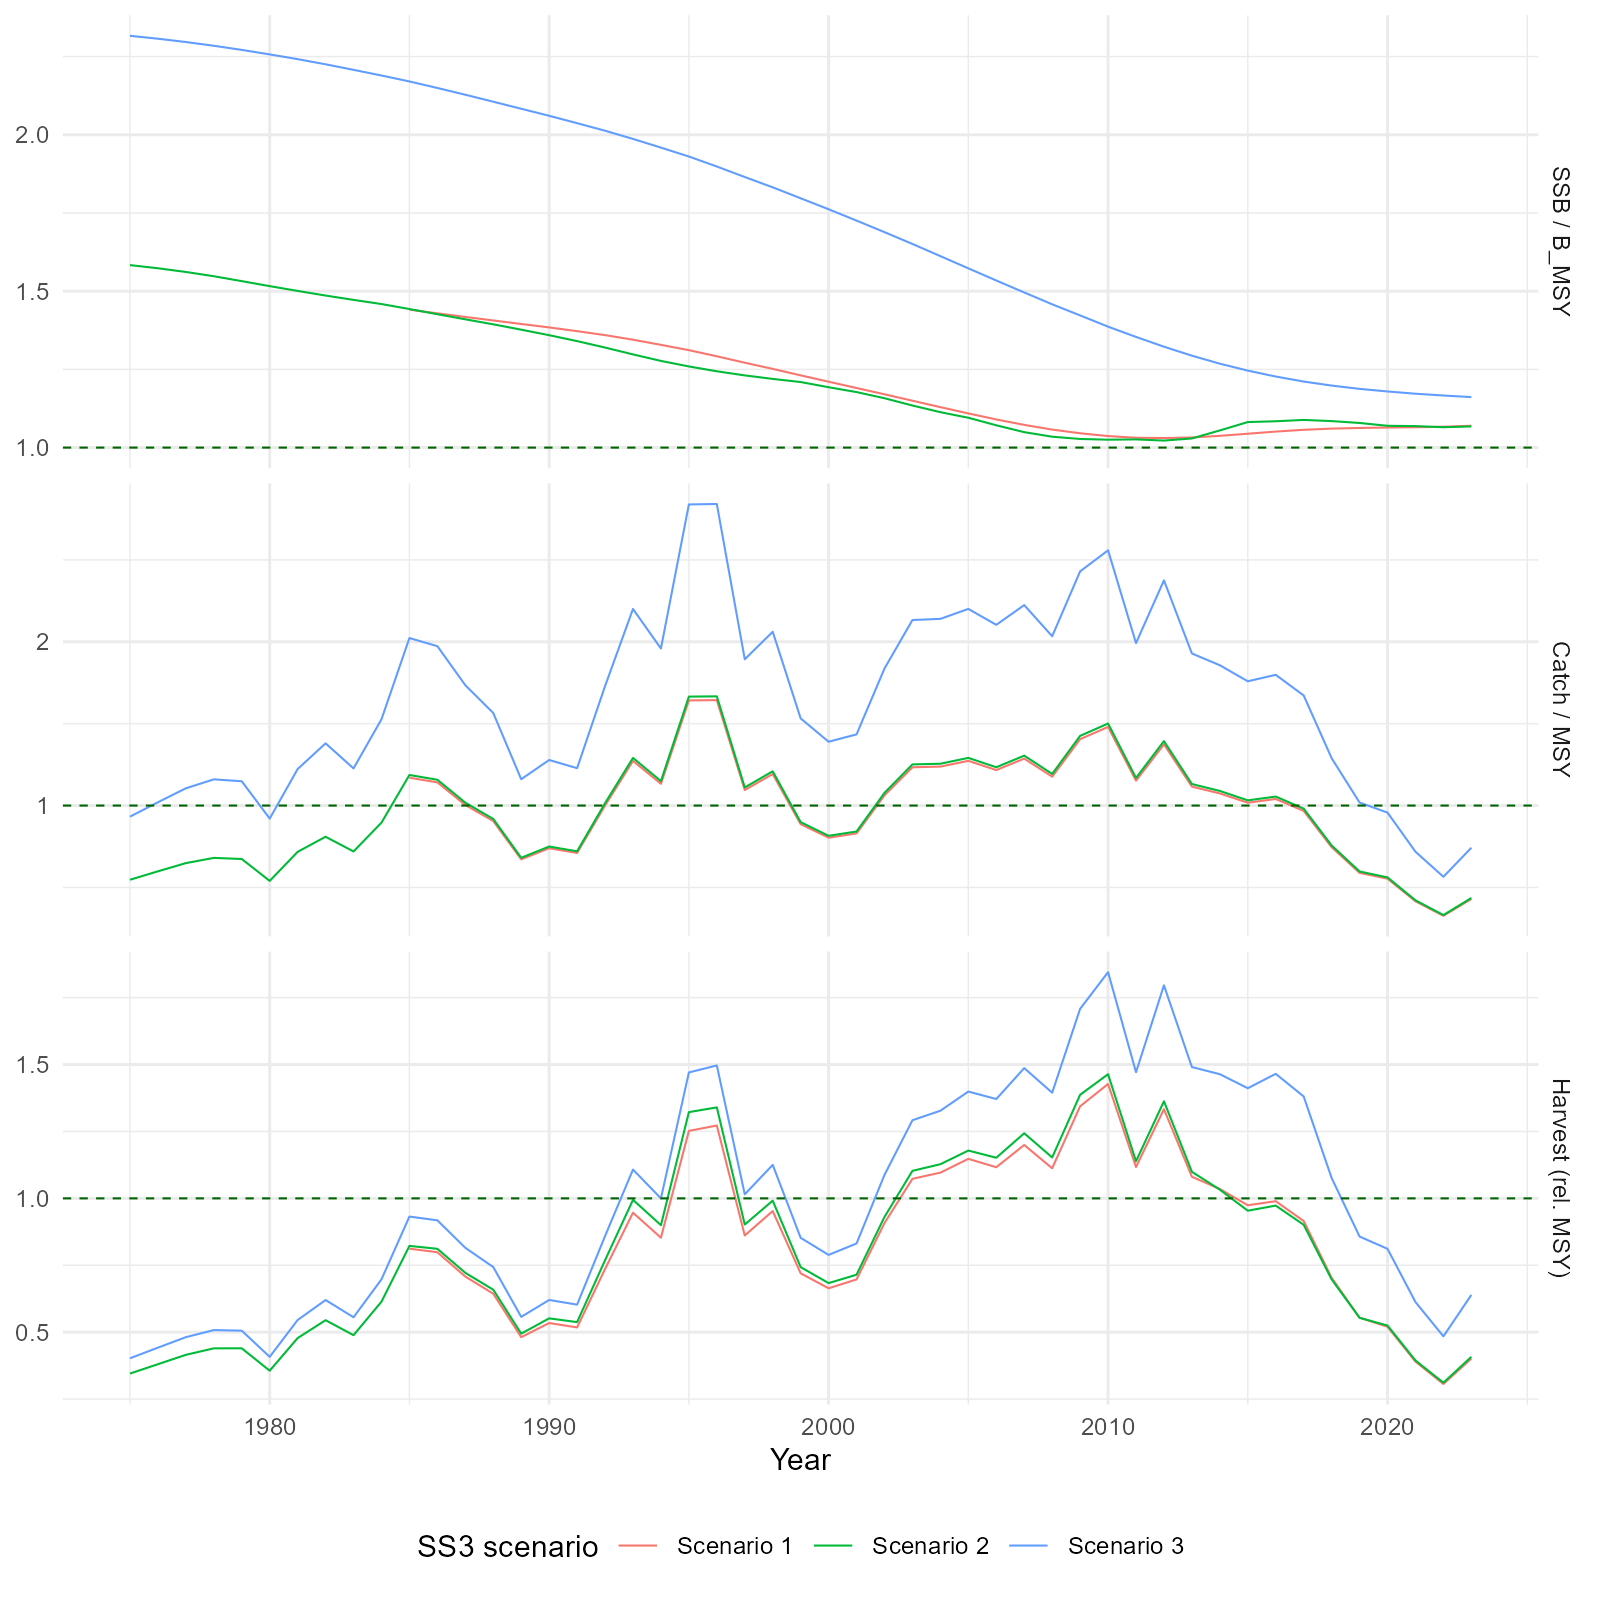
\includegraphics[width=0.92\linewidth]{figs/sma-fig-ts-1.png}
  \caption{sma fig ts 1}
  \label{fig:internal-sma-fig-ts-1}
\end{figure}

\begin{figure}[H]
  \centering
  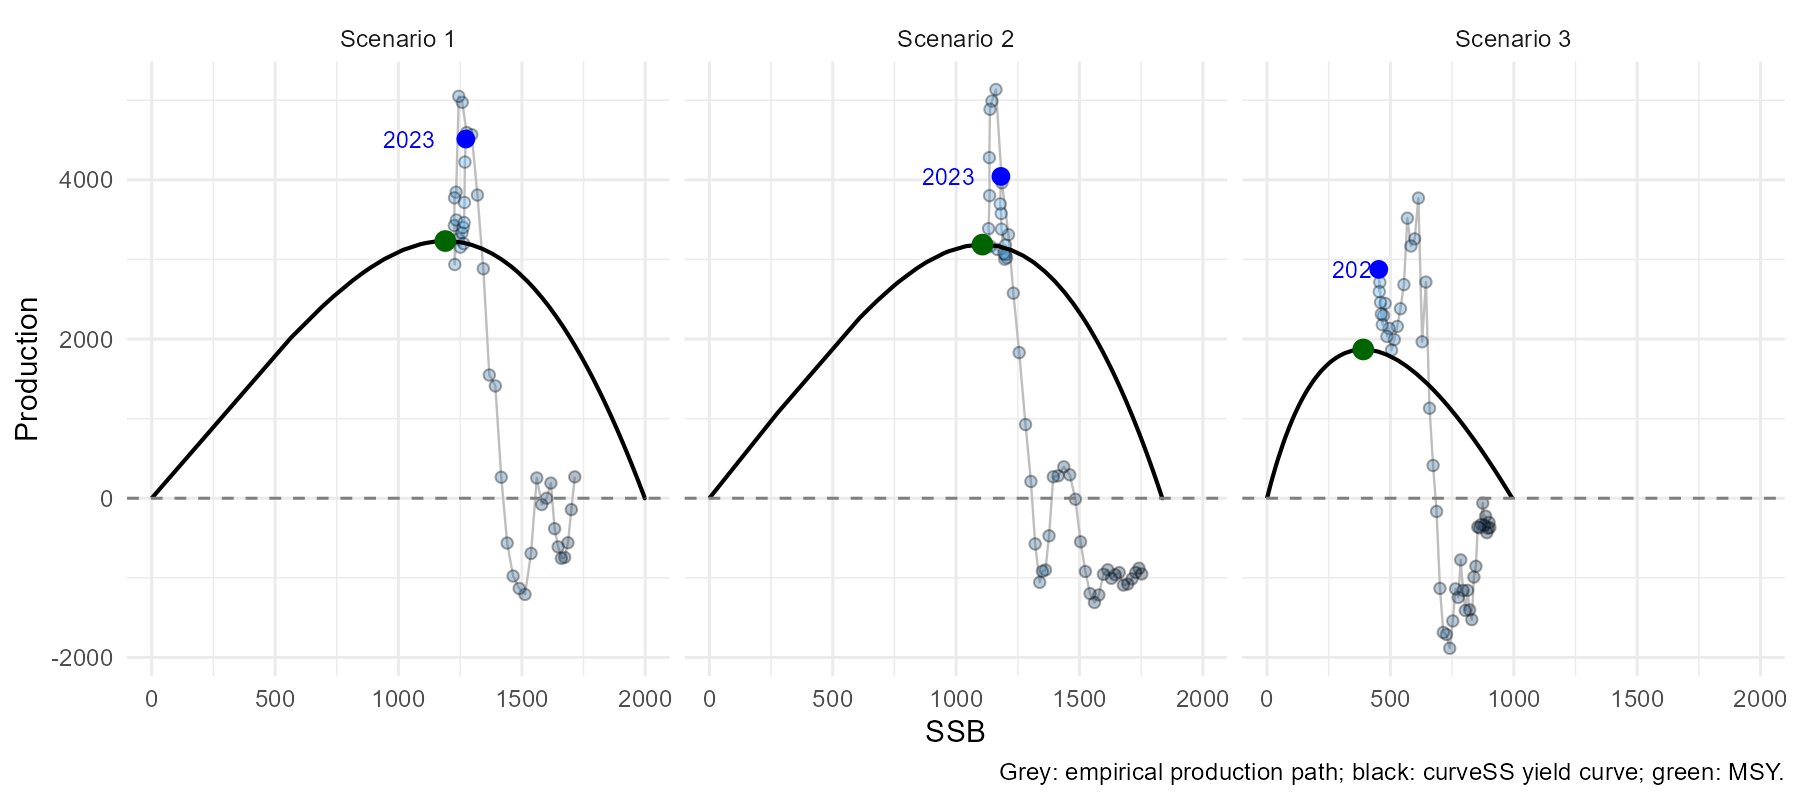
\includegraphics[width=0.92\linewidth]{figs/sma-fig-pe-phase-1.png}
  \caption{sma fig pe phase 1}
  \label{fig:internal-sma-fig-pe-phase-1}
\end{figure}

\begin{figure}[H]
  \centering
  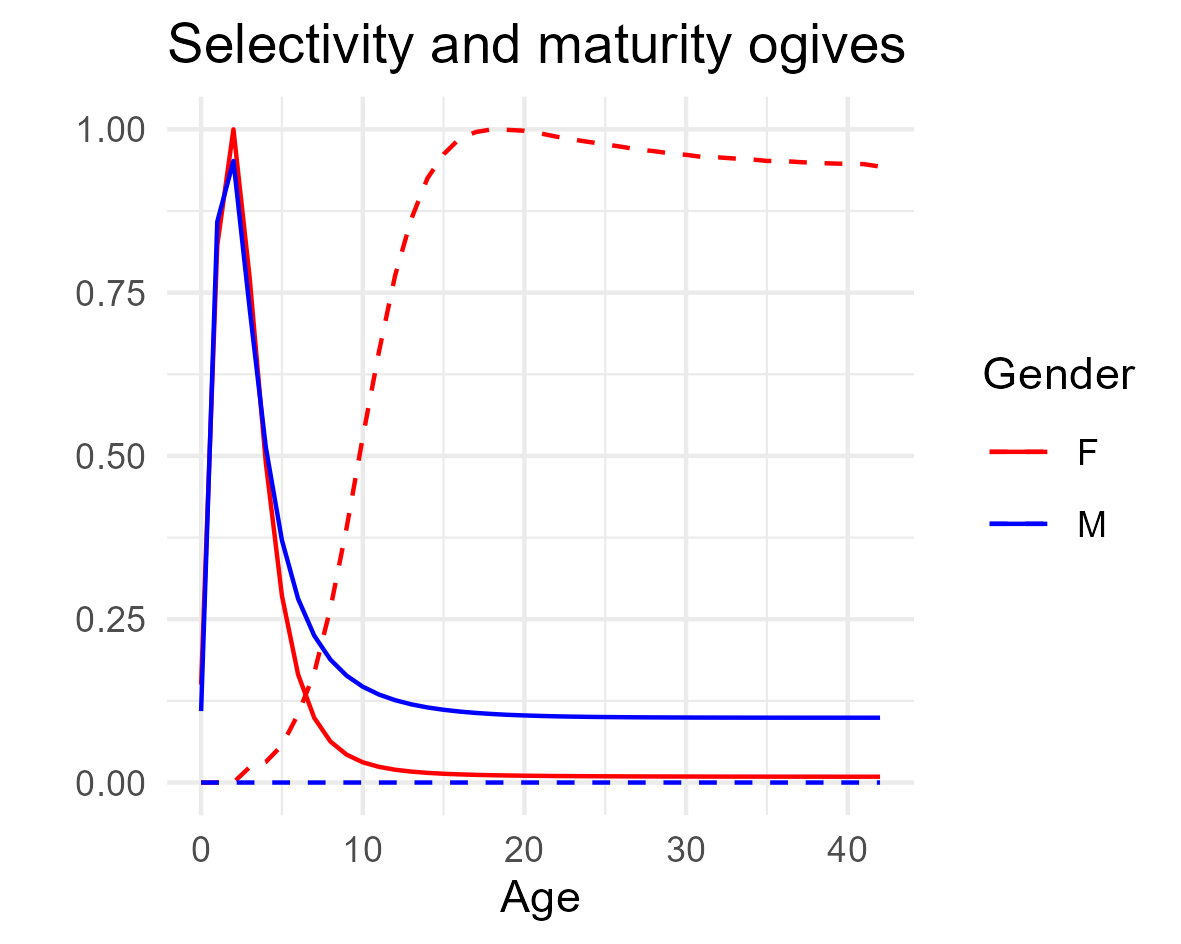
\includegraphics[width=0.92\linewidth]{figs/selmat.png}
  \caption{selmat}
  \label{fig:internal-selmat}
\end{figure}

\begin{figure}[H]
  \centering
  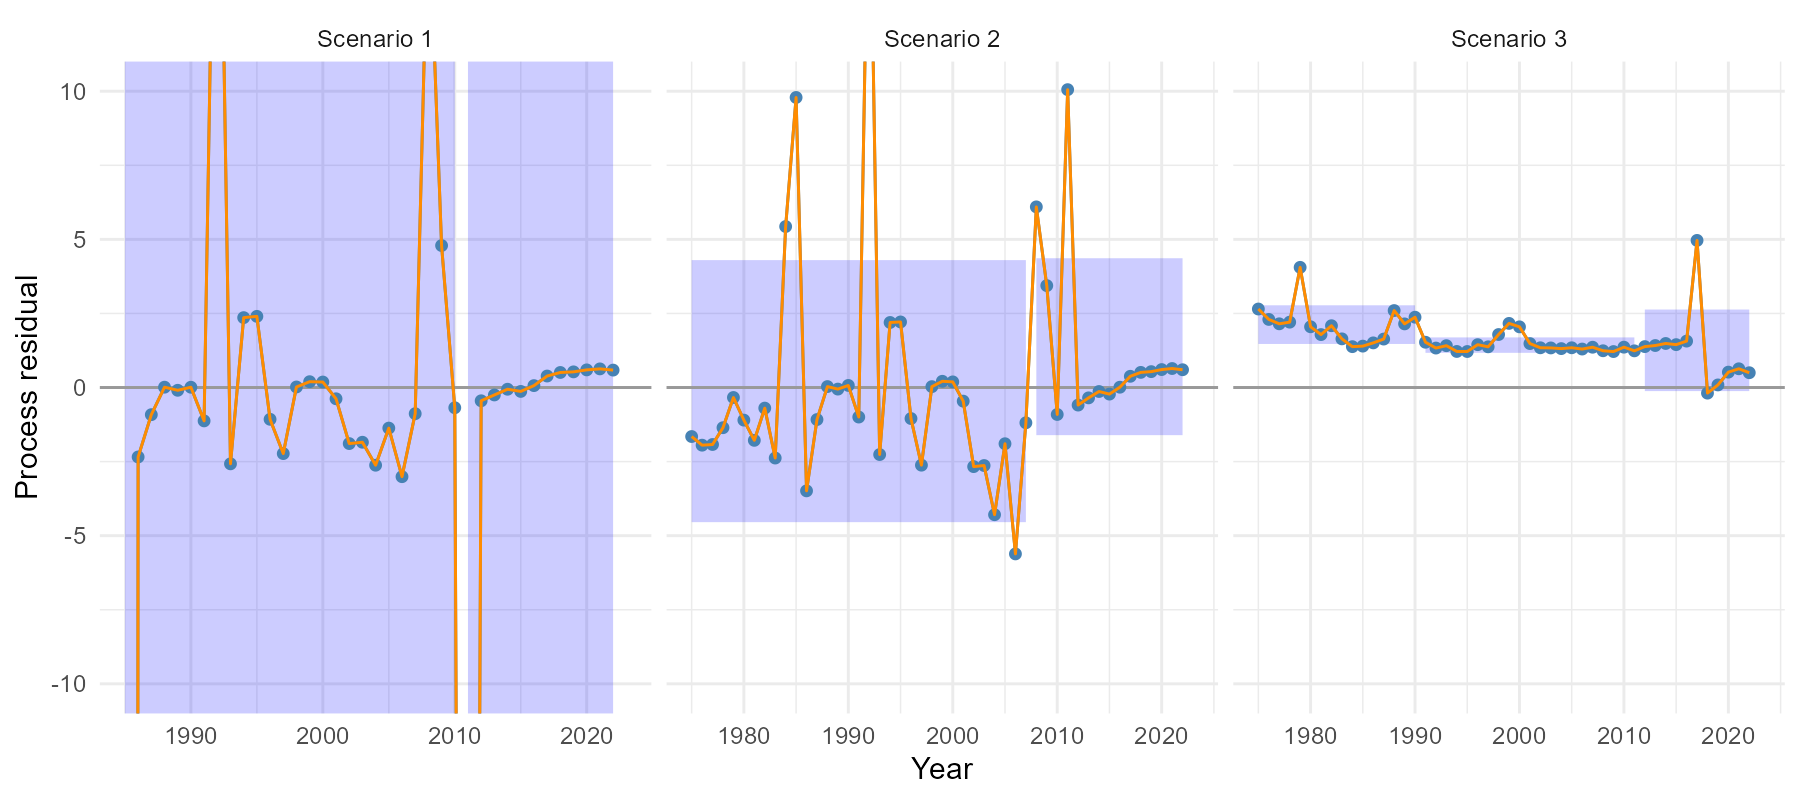
\includegraphics[width=0.92\linewidth]{figs/sma-fig-res-time-1.png}
  \caption{sma fig res time 1}
  \label{fig:internal-sma-fig-res-time-1}
\end{figure}

\begin{figure}[H]
  \centering
  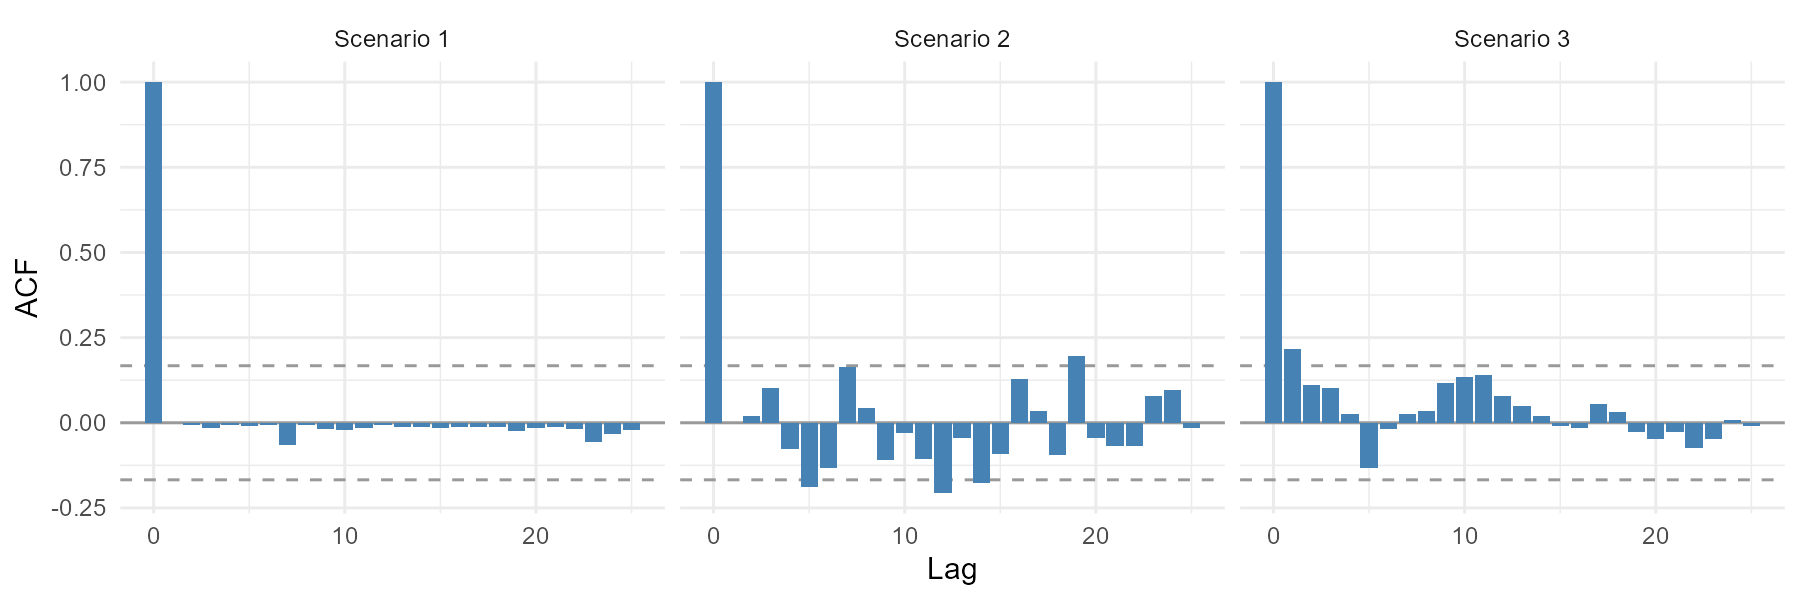
\includegraphics[width=0.92\linewidth]{figs/sma-fig-res-acf-1.png}
  \caption{sma fig res acf 1}
  \label{fig:internal-sma-fig-res-acf-1}
\end{figure}

\begin{figure}[H]
  \centering
  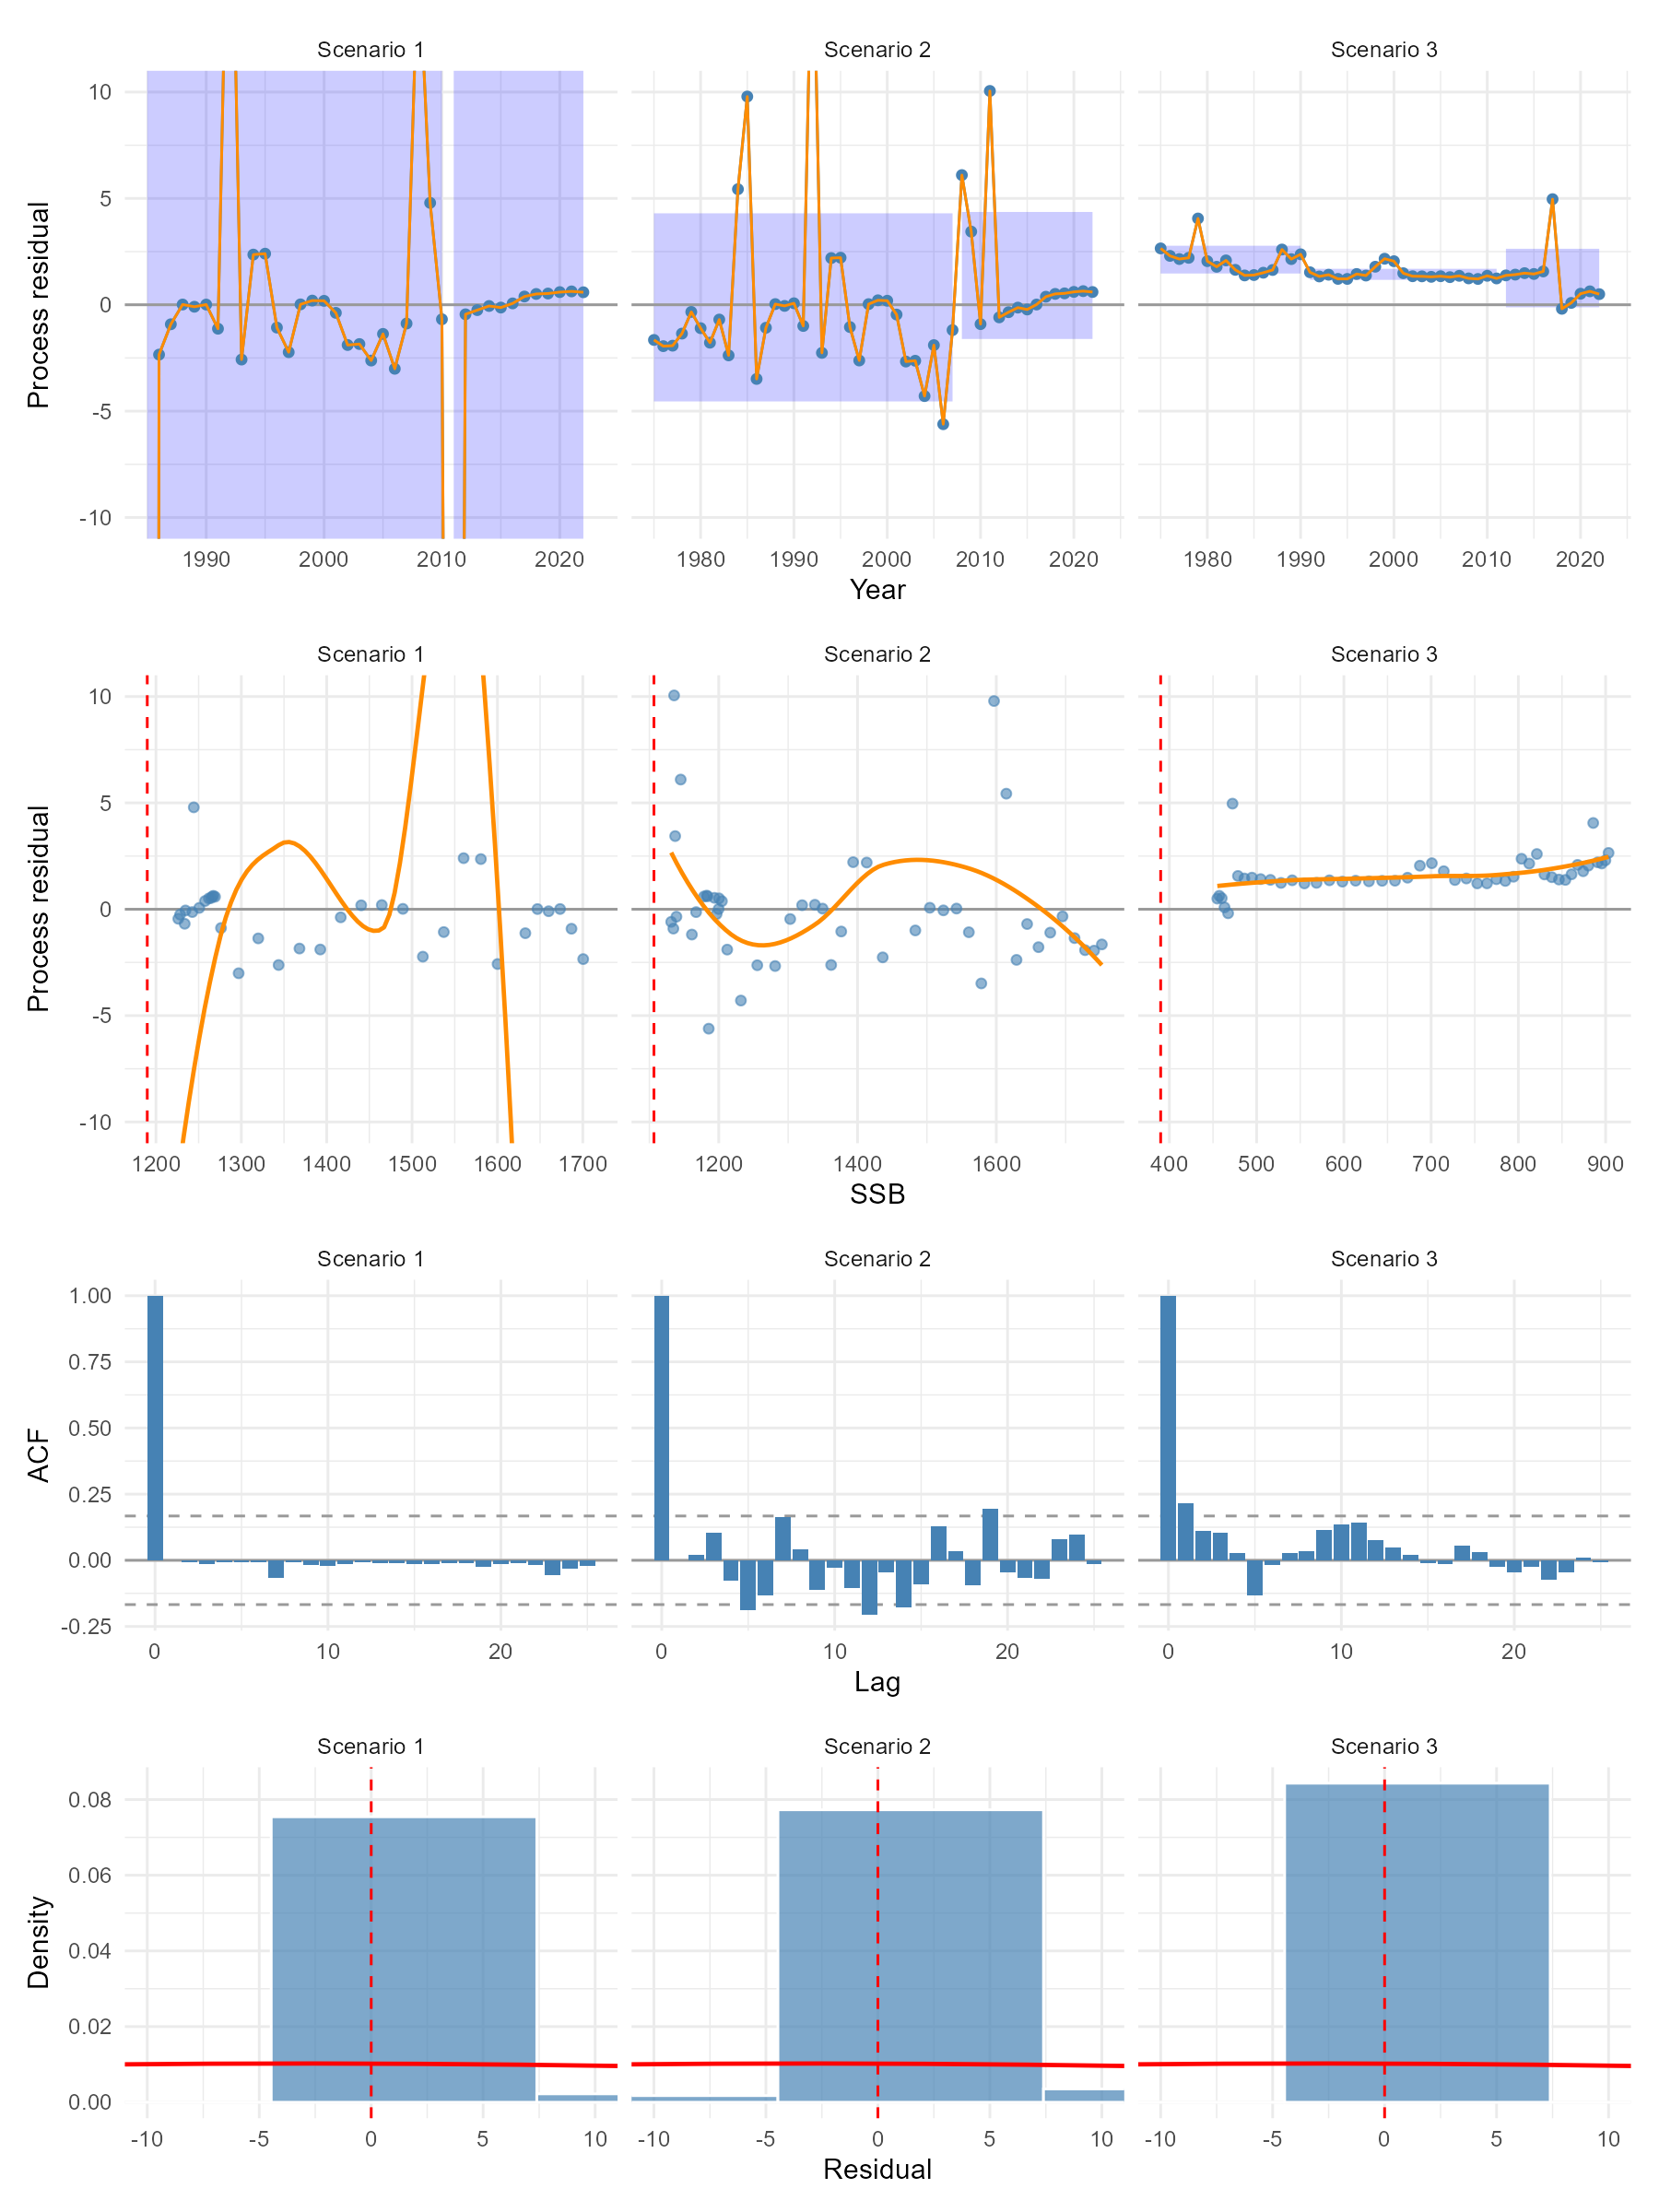
\includegraphics[width=0.92\linewidth]{figs/4panel.png}
  \caption{4panel}
  \label{fig:internal-4panel}
\end{figure}



\subsection{Interpretation}

Summarise whether the model is technically well fitted, which quantities are weakly
identified, and which issues should be carried forward to the robustness appendix.

% Case-specific internal interpretation.
% Summarise whether management quantities are informed by data,
% whether likelihood profiles or Hessian checks indicate weak identifiability,
% and which issues should be carried to the robustness appendix.


